\documentclass[10pt,aspectratio=169,serif]{beamer}

\usepackage[fontset=none, scheme=plain]{ctex}
\IfFontExistsTF{Songti SC}{%
	\setCJKmainfont{Songti SC}[AutoFakeSlant=0.2]%
	\setCJKsansfont{Songti SC}[AutoFakeSlant=0.2]%
}{%
	\setCJKmainfont{FandolSong-Regular}[Extension=.otf,BoldFont=FandolSong-Bold,AutoFakeSlant=0.2]%
	\setCJKsansfont{FandolSong-Regular}[Extension=.otf,BoldFont=FandolSong-Bold]%
}
\usepackage{amsmath,amssymb,graphicx,tikz,booktabs,multicol,calligra}
\usepackage{pgfplots}
\pgfplotsset{compat=1.18}
\usepackage{tcolorbox}
\tcbuselibrary{skins}
\usepackage{XyygU}
\usepackage{caption}
\captionsetup[figure]{name=图,labelsep=period}

\usetikzlibrary{arrows.meta,positioning,calc}

\setlength{\abovedisplayskip}{0pt plus 2pt minus 2pt}
\setlength{\belowdisplayskip}{0pt plus 2pt minus 2pt}

\title[习题5.7]{习题5.7 三角函数的应用}
\subtitle{综合运用 \& 拓广探索}
\author{}
\institute{}
\date{2026-10-16}

\begin{document}

\begin{frame}
  \titlepage
\end{frame}

% --- 1 ---
\begin{frame}[t]{第1题：造父变星亮度周期}
\textbf{1.} 天上有些恒星的亮度是会变化的，其中一种称为造父（型）变星，本身体积会膨胀收缩造成亮度周期性变化。下图是一造父变星的亮度随时间的周期变化图。此变星的亮度变化的周期为多少天？最亮时是几等星？最暗时是几等星？

\begin{center}
\begin{tikzpicture}[scale=0.9]
\begin{axis}[width=11cm,height=4.5cm,axis lines=middle,xlabel=$t$/天,ylabel=视星等,
xmin=0,xmax=20,ymin=3.4,ymax=4.6,xtick={0,1,2,3,4,5,6,7,8,9,10,11,12,13,14,15,16,17,18,19,20},
ytick={3.5,4.0,4.5},grid=major,grid style={gray!20}]
\addplot[thick,magenta,domain=0:20,samples=300] {4.0+0.5*cos(deg(360*(x-1)/5.5))};
\end{axis}
\end{tikzpicture}
\end{center}
\end{frame}

\begin{frame}[t]{第1题 解答}
\begin{tcolorbox}[colback=orange!10,colframe=orange,title=\textbf{解}]
相邻两次最亮（视星等最小）之间的时间约为 $5.5$ 天（如 $t\approx 1,6.5,12,17.5$）。

\alert{周期约为 $5.5$ 天}。

最亮时视星等约 $3.5$ 等星；最暗时视星等约 $4.5$ 等星。

\small（星等数越小越亮，故 $3.5$ 等比 $4.5$ 等亮。）
\end{tcolorbox}
\end{frame}

% --- 2 ---
\begin{frame}[t]{第2题：弹簧振子 $h=2\sin(t+\frac{\pi}{4})$}
\textbf{2.} 如图，弹簧挂着的小球做上下运动，它在 $t$ s 时相对于平衡位置的高度 $h$（单位：cm）由关系式 $h=2\sin\!\left(t+\dfrac{\pi}{4}\right)$ 确定。以 $t$ 为横坐标，$h$ 为纵坐标，画出这个函数在一个周期的闭区间上的图象，并回答：
\begin{enumerate}
  \item 小球在开始振动（即 $t=0$）时的位置在哪里？
  \item 小球的最高点和最低点与平衡位置的距离分别是多少？
  \item 经过多少时间小球往复运动一次？
  \item 每秒钟小球能往复振动多少次？
\end{enumerate}
\end{frame}

\begin{frame}[t]{第2题 解答}
\begin{tcolorbox}[colback=orange!10,colframe=orange,title=\textbf{解}]
(1) $t=0$ 时 $h=2\sin\dfrac{\pi}{4}=\sqrt2\approx 1.41$ cm，即在平衡位置上方 $1.41$ cm 处。

(2) 振幅 $A=2$，最高点和最低点到平衡位置距离都是 $2$ cm。

(3) $\omega=1$，周期 $T=\dfrac{2\pi}{1}=2\pi\approx 6.28$ s，即经过 $2\pi$ s 往复一次。

(4) 频率 $f=\dfrac1T=\dfrac1{2\pi}\approx 0.16$ 次/秒。
\end{tcolorbox}
\begin{center}
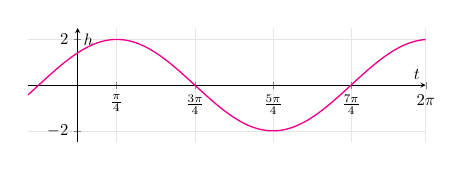
\begin{tikzpicture}[scale=0.6]
\begin{axis}[width=10cm,height=4cm,axis lines=middle,xlabel=$t$,ylabel=$h$,
xmin=-1,xmax=7,ymin=-2.5,ymax=2.5,xtick={0.78,2.36,3.93,5.5,7},xticklabels={$\frac{\pi}{4}$,$\frac{3\pi}{4}$,$\frac{5\pi}{4}$,$\frac{7\pi}{4}$,$2\pi$},
ytick={-2,2},grid=major,grid style={gray!20}]
\addplot[thick,magenta,domain=-1:7,samples=200] {2*sin(deg(x+pi/4))};
\end{axis}
\end{tikzpicture}
\end{center}
\end{frame}

% --- 3 ---
\begin{frame}[t]{第3题：天安门升旗时间（实践调查）}
\textbf{3.} 北京天安门广场的国旗每天是在日出时随太阳升起，在日落时降旗。请根据年鉴或其他参考资料，统计过去一年不同日期的日出和日落时间。
\begin{enumerate}
  \item 在同一直角坐标系中，以日期为横轴，画出散点图，并用曲线去拟合这些数据，同时找到函数模型；
  \item 某同学准备在五一长假时去看升旗，他应当在几点前到达天安门广场？
\end{enumerate}
\end{frame}

\begin{frame}[t]{第3题 解答（方法与参考）}
\begin{tcolorbox}[colback=orange!10,colframe=orange,title=\textbf{建模方法}]
(1) 日出（落）时间近似满足正弦型函数。以一年为周期，夏至（6月22日）日出最早、冬至（12月22日）日出最晚，故
\[
t_{\text{日出}}(d)=A\sin\!\left(\frac{2\pi}{365}(d-80)\right)+t_0,
\]
其中 $d$ 为一年中的第几天。北京地区 $t_0\approx 5:30$，振幅 $A\approx 2$ 小时。

(2) 五一（5月1日，约为年中第121天）北京日出约为 $5$ 时 $15$ 分左右。\alert{建议 $5$ 时前到达天安门广场}（实际以当日公告为准）。
\end{tcolorbox}
\end{frame}

% --- 4 ---
\begin{frame}[t]{第4题："削峰平谷"电价方案（开放实践）}
\textbf{4.} 夏天是用电高峰时期，特别在晚上。为保证居民空调制冷用电，电力部门不得不对企事业单位拉闸限电；而到了零时以后，又出现电力过剩。电力部门提出"削峰平谷"：提高晚上高峰时期电价，同时降低后半夜低峰时期电价，鼓励各单位在低峰时用电。请调查你们地区每天的用电情况，制定一项"削峰平谷"的电价方案。
\end{frame}

\begin{frame}[t]{第4题 解答（方案框架）}
\begin{tcolorbox}[colback=orange!10,colframe=orange,title=\textbf{参考方案}]
将一天按用电曲线（以 $24$ h 为周期的近似正弦曲线，峰值约在 $20:00$，谷值约在 $04:00$）分为三段：
\begin{itemize}
  \item \textbf{峰段}（$8{:}00$--$11{:}00$，$18{:}00$--$21{:}00$）：电价上浮 $50\%$；
  \item \textbf{平段}（其余日间）：执行基准电价；
  \item \textbf{谷段}（$22{:}00$--次日 $7{:}00$）：电价下浮 $50\%$，鼓励用电（充电、储能、生产）。
\end{itemize}
用 $P(t)=P_0+A\sin\!\left(\dfrac{2\pi t}{24}-\dfrac{7\pi}{6}\right)$ 拟合负荷曲线，按峰谷时段差引导需求侧响应。
\end{tcolorbox}
\end{frame}

\begin{frame}[c]
  \begin{center}
    {\Huge\calligra Thanks!}
  \end{center}
\end{frame}

\end{document}
